%\begin{minipage}{0.5\linewidth}
%	asdaegedf
%\end{minipage}\hfil
%\begin{minipage}{0.5\linewidth}
%	\begin{figure}[H]
%		%		\begin{flushright}
%		\resizebox{\textwidth}{!}{
%			\begin{tikzpicture}
%			% We start by placing the blocks
%			\node [box] (Geomagic) {\small{Geomagic Touch}};
%			\node [box, right of=Geomagic, node distance = 3.4cm] (Computer) {Computer};
%			\node [box, below of=Computer, node distance=3.3cm] (Sbrio) {Embedded\\System};
%			\node [box, left of=Sbrio, node distance=2.5cm] (Driver) {Motor driver};
%			\node [box, left of=Driver, node distance=2.5cm] (EndoWrist) {EndoWrist};
%			% We draw an edge between the controller and system block to
%			% calculate the coordinate u. We need it to place the measurement block.
%			\draw [<->] (Geomagic) -- node {} (Computer);
%			\draw [<->] (Computer) -- node {} (Sbrio);    
%			% \draw [<->] (Geomagic) -- node[label=above:\small{UDP}] {} (Computer);
%			% \draw [<->] (Computer) -- node [label=right:\small{UDP}] {} (Sbrio);
%			\draw [<->] (Sbrio) -- node {} (Driver);
%			\draw [->] (Driver) -- node {} (EndoWrist);
%			
%			\draw[thick,dashed] ($(-1.5,1)+(Geomagic)$) -- ($(1.5,1)+(Computer)$) -- ($(1.5,-1)+(Computer)$) -- ($(-1.5,-1)+(Geomagic)$)-- ($(-1.5,1)+(Geomagic)$);
%			\draw[thick,dashed] ($(-1.5,1)+(EndoWrist)$) -- ($(1.5,1)+(Sbrio)$) -- ($(1.5,-1)+(Sbrio)$) -- ($(-1.5,-1)+(EndoWrist)$)-- ($(-1.5,1)+(EndoWrist)$);
%			
%			\node at (2,1.7) {\textbf{Console}};
%			\node at (1.5,-2) {\textbf{da Vinci robot}};
%			
%			%\node [box, below of=Computer, node distance=3.3cm] (Sbrio) {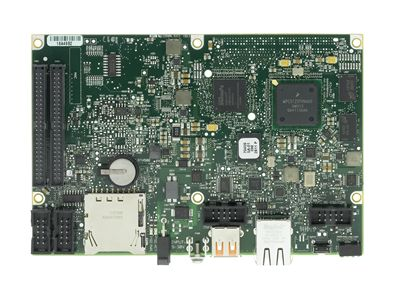
\includegraphics[width=.25\textwidth]{../Worksheets/rapport/pictures/sbRIO9636.jpg}};
%			\end{tikzpicture}
%			
%		}
%		%\end{flushright}
%		\caption{Block diagram representing the system.}
%		\label{fig:full_setup}
%	\end{figure}
%\end{minipage}

\begin{minipage}{\textwidth}
	\begin{figure}[H]
		\resizebox{\textwidth}{!}{
			\begin{tikzpicture}
			%\draw (-1.5,-2.5) rectangle (13.5,2.5);
			
			
			\node[box] (Opt) at (0,0) {\small Surgeon};
			\node[box] (Geo) at ($(3,0) + (Opt)$) {\small Haptic\\device};
			\node[box] (ros) at ($(3,0) + (Geo)$) {\small Robotic\\operating\\system};
			\node[box] (davin) at ($(3,0) + (ros)$) {\small Embedded \\system};
			\node[box] (end) at ($(3,0) + (davin)$) {\small End-effecor};
			
			
			\draw[->, ultra thick] ([yshift=0.3cm]Opt.east) -- ([yshift=0.3cm]Geo.west);
			\draw[->, ultra thick] ([yshift=0.3cm]Geo.east) -- ([yshift=0.3cm]ros.west);
			\draw[->, ultra thick] ([yshift=0.3cm]ros.east) -- ([yshift=0.3cm]davin.west);
			\draw[->, ultra thick] ([yshift=0.3cm]davin.east) -- ([yshift=0.3cm]end.west);
			
			
			\draw[<-, ultra thick] ([yshift=-0.3cm]Opt.east) -- ([yshift=-0.3cm]Geo.west);
			\draw[<-, ultra thick] ([yshift=-0.3cm]Geo.east) -- ([yshift=-0.3cm]ros.west);
			\draw[<-, ultra thick] ([yshift=-0.3cm]ros.east) -- ([yshift=-0.3cm]davin.west);
			%\draw[<-, ultra thick] ([yshift=-0.3cm]davin.east) -- ([yshift=-0.3cm]end.west);
			
			\node at (1.5,1) {Position};
			\node at (4.5,1) {Position};
			% \node at (7.5,1) {yes};
			% \node at (10.5,1) {yes};
			
			\node at (1.5,-1) {\small Force};
			\node at (4.5,-1) {\small Force};
			\node at (10.5,1) {\small Torque};
			% \node at (10.5,1) {yes};
			\node at (7.5,1.2) {\small Motor enable};
			\node at (7.5,0.8) {\small Position};
			\node at (7.5,-0.8) {\small Position};
			\node at (7.5,-1.2) {\small Speed};
			\node at (7.5,-1.6) {\small Current};
			
			\end{tikzpicture}
		}
		\footnotesize\caption{System overview}
		\label{fig:overview}
	\end{figure}
\end{minipage}\hfil


\begin{minipage}{\textwidth}
The test system shown on \figref{fig:overview} controls the da Vinci end-effector detached from the system.
The control structure has high computation demand therefore a computer running the robotic operating sytem (ROS) is added to the system.
% The control structure presented on ----------- has high computation demand which cannot be satisfied by the embedded system. Therefore the haptic device needs to interface with the embedded system through a computer running the robotic operating sytem (ROS), that also provides the required computation power.
\end{minipage}


